% This file was created by matlab2tikz.
%
%The latest updates can be retrieved from
%  http://www.mathworks.com/matlabcentral/fileexchange/22022-matlab2tikz-matlab2tikz
%where you can also make suggestions and rate matlab2tikz.
%

\documentclass[10pt]{standalone}
\usepackage{amsmath}
\usepackage{graphicx}
\usepackage[pdf]{pstricks}
\usepackage{pgfplots}
\pgfplotsset{compat=newest}
\usepgfplotslibrary{fillbetween}
%% the following commands are needed for some matlab2tikz features
\usetikzlibrary{plotmarks}
\usetikzlibrary{arrows.meta}
\usepgfplotslibrary{patchplots}
\usetikzlibrary{decorations.text}
\usetikzlibrary{shapes.multipart}

\begin{document}
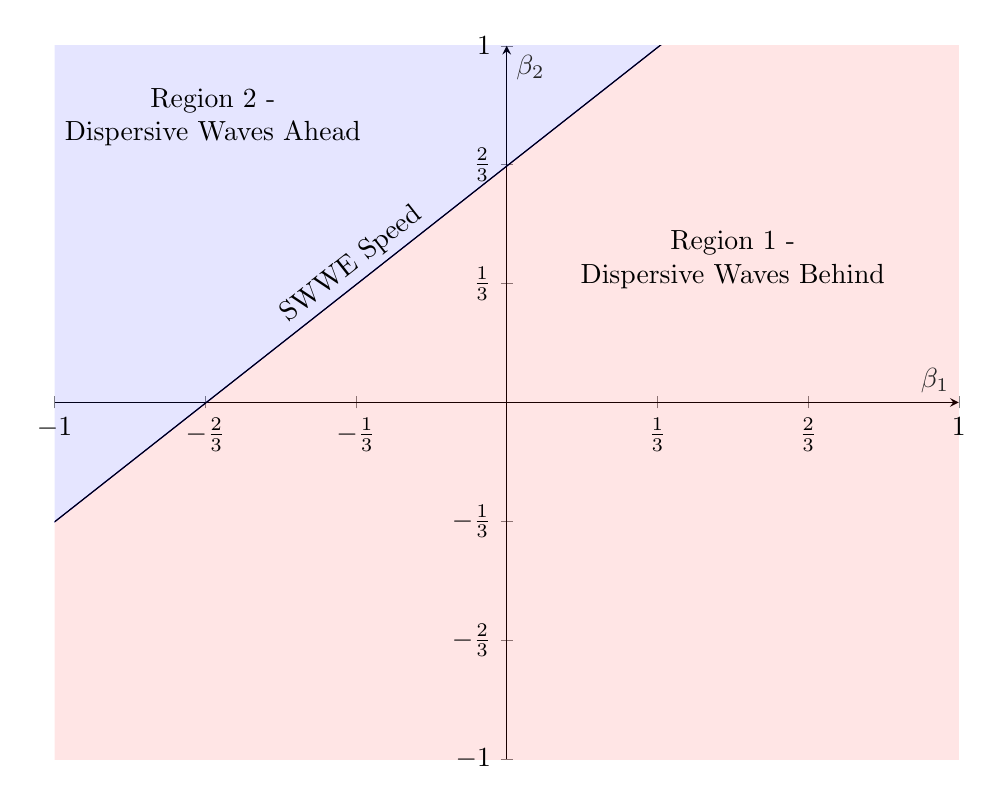
\begin{tikzpicture}[every text node part/.style={align=center}]

\begin{axis}[%
width=4.521in,
height=3.566in,
at={(0.758in,0.481in)},
scale only axis,
axis lines=center,
xmin=-1,
xmax=1,
xtick={-1,-0.66666,-0.33333,0.33333,0.66666,1},
xticklabels = {$-1$,$-\frac23$,$-\frac13$,$\frac13$,$\frac23$,$1$},
xlabel style={font=\color{white!15!black}},
xlabel={$\beta_1$},
ymin=-1,
ymax=1,
ytick={-1,-0.66666,-0.33333,0.33333,0.66666,1},
yticklabels = {$-1$,$-\frac23$,$-\frac13$,$\frac13$,$\frac23$,$1$},
ylabel style={font=\color{white!15!black}},
ylabel={$\beta_2$},
axis background/.style={fill=white},
];
\addplot+[name path=Above,mark=none, white] coordinates {(-2,2) (2,2)};
\addplot+[name path=Critical,mark=none, blue] coordinates {(-1.66666,-1) (1,1.66)};
\addplot[decoration={text along path,
	text={SWWE Speed},
	raise=1ex,
	text align={left indent={0.45\dimexpr\pgfdecoratedpathlength\relax}}},
postaction={decorate}]
coordinates {(-1.66666,-1) (1,1.66)};


\addplot+[name path=Below,mark=none, white] coordinates {(-2,-2) (2,-2)};
\addplot[blue,opacity=0.1] fill between[of=Above and Critical];
\addplot[red,opacity=0.1] fill between[of=Critical and Below];

\node[] at (axis cs: 0.5,.4) {Region 1 - \\ Dispersive Waves Behind};
\node[] at (axis cs: -0.65,0.8) {Region 2 - \\ Dispersive Waves Ahead};
\end{axis}

\end{tikzpicture}%

\end{document}